\documentclass[12pt, a4paper]{article} 
 
\usepackage[utf8]{inputenc}
 
 
\usepackage{geometry} % to change the page dimensions
\geometry{a4paper} % or letterpaper (US) or a5paper or....
 
\usepackage{graphicx} % support the \includegraphics command and options

\usepackage{booktabs} % for much better looking tables
\usepackage{array} % for better arrays (eg matrices) in maths
\usepackage{paralist} % very flexible & customisable lists (eg. enumerate/itemize, etc.)
\usepackage{verbatim} % adds environment for commenting out blocks of text & for better verbatim
\usepackage{subfig} % make it possible to include more than one captioned figure/table in a single float
% These packages are all incorporated in the memoir class to one degree or another...
 \usepackage{import} % for importing other .tex files
 
\usepackage{color} 
\usepackage{amsmath, amssymb}% for mathematical symbols

\definecolor{gray}{rgb}{0.5,0.5,0.5}
\usepackage[colorlinks=true,linkcolor=black, citecolor=gray, urlcolor = blue]{hyperref} % for hyperreferences with black color
\usepackage[T1]{fontenc} % Uncomment for norwegian document
%\usepackage[norsk]{babel} %




 
%%% HEADERS & FOOTERS
\usepackage{fancyhdr} % This should be set AFTER setting up the page geometry
\pagestyle{fancy} % options: empty , plain , fancy
\renewcommand{\headrulewidth}{0pt} % customise the layout...
\lhead{}\chead{}\rhead{}
\lfoot{}\cfoot{\thepage}\rfoot{}
 
%%% SECTION TITLE APPEARANCE
\usepackage{sectsty}
\allsectionsfont{\sffamily\mdseries\upshape} % (See the fntguide.pdf for font help)
% (This matches ConTeXt defaults)
 
%%% ToC (table of contents) APPEARANCE
\usepackage[nottoc,notlof,notlot]{tocbibind} % Put the bibliography in the ToC
\usepackage[titles,subfigure]{tocloft} % Alter the style of the Table of Contents
\renewcommand{\cftsecfont}{\rmfamily\mdseries\upshape}
\renewcommand{\cftsecpagefont}{\rmfamily\mdseries\upshape} % No bold!

%%%Code

\definecolor{bluekeywords}{rgb}{0.13,0.13,1}
\definecolor{greencomments}{rgb}{0,0.5,0}
\definecolor{redstrings}{rgb}{0.9,0,0}

\usepackage{listings}
\lstset{language=[Sharp]C,
showspaces=false,
showtabs=false,
breaklines=true,
showstringspaces=false,
breakatwhitespace=true,
escapeinside={(*@}{@*)},
commentstyle=\color{greencomments},
keywordstyle=\color{bluekeywords}\bfseries,
stringstyle=\color{redstrings},
basicstyle=\ttfamily
}
 
%stuff to refer/cite

\usepackage[sort]{natbib}

 
%%% END Article customizations
 
%%% The "real" document content comes below...
 
\title{\normalsize Customer driven project, TDT4290 \\ \LARGE \textbf{Automatic Import of Completed Ads} \normalsize \\Adresseavisen AS}
\author{Audun Skjervold \\ Erlend Løkken Sigholt \\ Truls Hamborg \\ Hong-Dang Lam}
%\date{} % Activate to display a given date or no date (if empty),
         % otherwise the current date is printed 
 
\begin{document}
\maketitle 
\newpage
\tableofcontents
\newpage

\chapter*{Abstract}

This paper describes the process of developing a framework for Automatic Importing of Completed Ads, on request from Adresseavisen AS, which is a major regional newspaper. It will describe the project, from the preliminary study phase and project management/organization, to implementation and completion.

The goal is to create a framework which will facilitate automatic importing of completed real estate ads in the form of pdf-files and associated data, with the possibility to expand to other types of ads. The accompanying data will be placed into the internal database of Adresseavisen and their internal order system for ads, and the pdf is to be saved in their archives.

Adresseavisen, as a customer, is interested in the framework in itself, with accompanying developer documentation for possible further development. In addition to this, we will produce full documentation of the process as a deliverable in the course which this project is for.

\chapter*{Preface}
This document was written for the project-based course \em TDT4290 Customer Driven Project\em, at the \em Norwegian University of Technology and Science, NTNU\em \ during the fall semester of 2013.

The project team consisted of four students from \em Computer Science \em  at the \em Department of Computer and Information Science\em \ at \em NTNU\em. The project was \em Automated Import of Completed Ads\em, on behalf of \em Adresseavisen AS\em.

The team would like to thank customer representative Asle Dragsteen Liebech for great support and technological guidance, as well as our supervisor Zhu Meng for excellent supervising.
 
\chapter{Introduction}
This chapter gives a brief introduction to our project, including the customer, project purpose, project background, problem description among other subjects. 
\newpage

\section{Project name - Automatic Import of Completed Ads}
The project is named \em Automated Import of Completed Ads\em \ by the \\
customer; \em Adressavisen AS.\em \ The team is to create a framework for automatic import of real estate ads into Adresseavisen's internal database and order system.
\section{Customer - Adresseavisen AS}
Adresseavisen is a regional newspaper in Trondheim, Norway and the surrounding area. It publishes it's newspaper in Trøndelag and Nordmøre on a daily basis except on Sundays. It is an independent, conservative newspaper with a daily circulation of approximately 85000 NOK. 
Stocks in Adresseavisen are traded on the Oslo Stock Exchange.\\
\\
"In addition to the main newspaper, Adresseavisen owns several smaller local newspapers in the Trøndelag region. They also own and operate a local radio station, Radio-Adressa, and a local TV station, TV-Adressa (prior to 30 January 2006: TVTrøndelag). They also have a stake in the national radio channel Kanal 24. In addition, the newspaper owns the local newspapers Fosna-Folket, Hitra-Frøya, Levanger-Avisa, Sør-Trøndelag, Trønderbladet and Verdalingen." \cite{adressaWiki}

\section{Project Purpose}
The purpose of this project is to create a framework for automated import of complete ads in the form of pdf-files. The pdf-files will be accompanied by data, which shall be added to the database and used to create an order in Adresseavisens internal order system for ads. This framework will also be able to provide customers with certain information that is to be supplied when they wish to have an ad featured in Adresseavisen, such as available dates and ad-packages.

\section{Project Background}
Adresseavisen currently uses a system where ads to be featured on their website or published in newspapers are created in their internal order system, with the use of one of very many templates. This is very complex and an increasing amount of customers use their own fully completed ads, in the form of pdf-files.

Adresseavisen now has the need for a system which can automate and simplify the process of receiving these ads into the system, with the purpose of eventually replacing the old system.

\section{Problem Description}
Our plug-in to Webassistenten will take a completed ad in the form of a pdf file and save it to the appropiate folder. These folders will have the ID of the customer so that Adressa can easily identify which pdf belongs to which customer.

Webassistenten will require certain data along with the pdf, such as date to publish, module type (what kind of format it should be printed as in the newspaper) and which newspaper it will be printed in (known as product). In the case of real estate ads, the required data also includes locations, zip code, zip area, address, responsible realtor, phone number of aforementioned realtor, email etc. These data will be saved into a database internally in their system. 

\section{Existing Technology}
There currently exists no technology equivalent to ours that we are aware of. The technology that Adressa uses today in Webassistenten is different from the product we're developing for them in that the current solution doesn't accept a pdf as input. Instead it takes in pictures in addition to the accompanying data, and generates a pdf based on this input.

The already existing alternative that Webassistenten utilizes isn't as automated as they would like it to be, and the real estate agents might not get the perfectly designed ad in the pdf through this auto-generation.
%<Already existing technology that the customer could have used rather than employing us to develop new software. This is where we will write that we found no such technology and how we found that information.> %TODO

\section{Stakeholders}
\subsection{Customer}
Customer: Adresseavisen AS

\begin{table}[H]
\begin{tabular}{|l|l|}
\hline
\textbf{Name} & \textbf{E-mail} \\
\hline
Asle Dragsten Liebech & \href{mailto://asle.dragsten.liebech@adresseavisen.no}{asle.dragsten.liebech@adresseavisen.no}\\
Jostein Danielsen & \href{mailto://jostein.danielsen@adresseavisen.no}{jostein.danielsen@adresseavisen.no}\\
\hline
\end{tabular}
\caption{Customer Representatives}
\end{table}

The customer is, along with our group, the most important stakeholder of our project. The project supplies the customer with a product that hopefully will improve their business, as well as saving them money they would otherwise have had to spend developing the product themselves.

It is important for the customer that we have a successful project resulting in a good product because delivering a poor product would require unnecessary work on their end.
\subsection{Group Members}
\begin{table}[H]
\begin{tabular}{|p{5cm}|p{6cm}|}
\hline
\textbf{Name} & \textbf{E-mail} \\
\hline
Audun Skjervold & \href{mailto://audunskj@stud.ntnu.no}{audunskj@stud.ntnu.no}\\
Erlend Løkken Sigholt & \href{mailto://erlendsi@stud.ntnu.no}{erlendsi@stud.ntnu.no}\\
Hong-Dang Lam & \href{mailto://hongdang@stud.ntnu.no}{hongdang@stud.ntnu.no}\\
Truls Hamborg & \href{mailto://trulsbjo@stud.ntnu.no}{trulsbjo@stud.ntnu.no}\\
\hline
\end{tabular}
\caption{Group Members}
\end{table}

The members of our group are the other most important stakeholders of the project. This is mainly because the course gives course credit equivalent to two regular courses, making it more important to achieve a good grade.

\subsection{Course Staff}
\begin{table}[H]
\begin{tabular}{|p{4cm}|p{4cm}|p{5cm}|}
\hline
\textbf{Name} & \textbf{Role} & \textbf{E-mail} \\
\hline
Meng Zhu & Group Supervisor & \href{mailto://zhumeng@idi.ntnu.no}{zhumeng@idi.ntnu.no}\\
\hline
Reidar Conradi & Course Responsible & \href{mailto://conradi@idi.ntnu.no}{conradi@idi.ntnu.no}\\
\hline
\end{tabular}
\caption{Course Staff}
\end{table}

The course staff are the final stakeholders. The staff wants satisfied customers, and they want the students who participate in the course to achieve good results. To accomplish this, we need to deliver a well written report with good documentation of the project. We also need to keep our supervisor satisfied throughout the project, supplying him with good under-way documentation.

\section{Measure of Project Effects}
The completed ads produced through our product will in theory not be distinguishable from completed ads produced without it, although the design might differ from the auto-generated versions that would otherwise have been made. For this reason, we do not expect to see any effects of this project.

We do however hope that Adressa and their customers will see effects in the form of time and money saved. We also believe that the real estate agents to a larger extent will find the submitted ads being accepted in the format and design they want them to be.

\section{Duration}
The introduction to the course started on Wednesday 21.08.2013 when we all met in S6 for information and were introduced to the customer and the project.

The final delivery is three months after the course start, on 21.11.2013, at which point we will have a short 45 minute presentation where we introduce the product and our experience with this course.

\section{Project Management}
\subsection{Terms and Resources}
\subsection{Project Organization}
\subsection{Roles}
\documentclass[12pt, a4paper]{article} 
 
\usepackage[utf8]{inputenc}
 
 
\usepackage{geometry} % to change the page dimensions
\geometry{a4paper} % or letterpaper (US) or a5paper or....
 
\usepackage{graphicx} % support the \includegraphics command and options
 
\usepackage{booktabs} % for much better looking tables
\usepackage{array} % for better arrays (eg matrices) in maths
\usepackage{paralist} % very flexible & customisable lists (eg. enumerate/itemize, etc.)
\usepackage{verbatim} % adds environment for commenting out blocks of text & for better verbatim
\usepackage{subfig} % make it possible to include more than one captioned figure/table in a single float
% These packages are all incorporated in the memoir class to one degree or another...
 
 
 
\usepackage{amsmath, amssymb}% for mathematical symbols
\usepackage[colorlinks=true,linkcolor=black]{hyperref} % for hyperreferences with black color
%\usepackage[T1]{fontenc} % Uncomment for norwegian document
%\usepackage[norsk]{babel} %
 
%%% HEADERS & FOOTERS
\usepackage{fancyhdr} % This should be set AFTER setting up the page geometry
\pagestyle{fancy} % options: empty , plain , fancy
\renewcommand{\headrulewidth}{0pt} % customise the layout...
\lhead{}\chead{}\rhead{}
\lfoot{}\cfoot{\thepage}\rfoot{}
 
%%% SECTION TITLE APPEARANCE
\usepackage{sectsty}
\allsectionsfont{\sffamily\mdseries\upshape} % (See the fntguide.pdf for font help)
% (This matches ConTeXt defaults)
 
%%% ToC (table of contents) APPEARANCE
\usepackage[nottoc,notlof,notlot]{tocbibind} % Put the bibliography in the ToC
\usepackage[titles,subfigure]{tocloft} % Alter the style of the Table of Contents
\renewcommand{\cftsecfont}{\rmfamily\mdseries\upshape}
\renewcommand{\cftsecpagefont}{\rmfamily\mdseries\upshape} % No bold!

\begin{document}

\section{Roles}
\begin{itemize}
\item Scrum Master/Process responsible: Truls
\item Documentation Manager: Truls
\item Product Owner: Adresseavisen
\item Customer/Supervisor contact: HD
\item Administrator/Project Leader, System Architect: HD
\item Lead Coder, Project Lead: Erlend
\item Secretary: Erlend
\item Implementation manager: Audun
\end{itemize}


Test Manager: Everyone is responsible for testing their own code.


\end{document}
\subsection{Time schedule}
\subsection{Overall project plan}
\subsection{Risk Analysis}
\subsection{Issues}
The project didn't go as smoothly as we had hoped. The group agreed on pretty much everything, but the issues we had were mostly related to the software and tools not cooperating or working as we expected.

\subsubsection{C\# Compiler}
C\# compiler was not found due to uninstallìng of RC, this lead to the "add new" window not opening, and therefore not possible to add the entity framework.\\
This command in cmd fixed it:
\begin{verbatim}
gacutil /u Microsoft.VisualStudio.CSharp.Services.Language.Interop 
\end{verbatim}

\subsubsection{GitHub DDoS}
On October 14, the day of the midterm delivery, GitHub experienced a DDoS attack. This resulted in some of the files we were working on for the report becoming locked mid-commit and mid-pull, and preventing us from performing a new git pull. This also prevented some of us from compiling, due to a previous commit containing errors having been pulled.

\subsubsection{Windows on Mac}
Mac is not Windows. %TODO Truls

\subsubsection{SDM}
SDM %TODO HD? "Unkown error" thingy?

\subsubsection{MSSQL}
DB



The project didn't go as smooth as we had hoped for. The group agreed on pretty much everything, but the issues we had was mostly related to the software and tools not cooperating.
%Risks

\subsection{Internal Risks}
\subsubsection{Low experience with the development process}
\begin{tabular}{| l | l |}
	\hline
	What: & The group doesn't have much experience with lengthy projects\\
	\hline
	Probability: & High \\
	\hline
	Impact: & Low-High \\
	\hline
	Action: & Reduce by regularly reviewing progress and making use of \\
			& supervisor meetings etc.\\
	\hline

\end{tabular}

\subsubsection{Unfamiliarity with technology}
\begin{tabular}{| l | l |}
	\hline
	What: & Some members of the group have no experience with the \\
		& programming language in use, and only one has used the \\
		& relevant framework. Will require extra time for learning.\\
	\hline
	Probability: & Moderate \\
	\hline
	Impact: & Low-Moderate \\
	\hline
	Action: & Reduce by group members with experience \\
	& coaching others in the relevant technology\\
	& and practices. Set time aside for learning.\\
	\hline

\end{tabular}

\subsubsection{Unfamiliarity with tools}
\begin{tabular}{| l | l |}
	\hline
	What: & Some members of the group have no experience with\\
	& the tools we're using, it's complicated to\\
	& install due to the different versions of the tools \\
	& \& there's so many tools needed to start.\\
	\hline
	Probability: & Moderate \\
	\hline
	Impact: & Low-Moderate \\
	\hline
	Action: & Reduce by group members with experience \\
	& coaching others in the relevant technology\\
	& and practices. Set time aside for learning.\\
	& Debugging via Google.\\
	\hline

\end{tabular}




\subsubsection{Illness}
\begin{tabular}{| l | l |}
	\hline
	What: & As winter approaches, the probability of group members becoming \\	 & ill increases. Being a small group, this might be critical.\\
	\hline
	Probability: & Moderate \\
	\hline
	Impact: & Low-High \\
	\hline
	Action: & Do not tailgate deadlines. Work steadily, and have margins\\
	&and practices. Expect some members to not produce at 100\%\\	& every week.\\
	\hline

\end{tabular}

\subsubsection{Other engagements}
\begin{tabular}{| l | l |}
	\hline
	What: & Group members have extracurricular activities that require time \\
	 & certain dates during the semester.\\
	 & This might cause absence and/or reduced work-output.\\
	\hline
	Probability: & Moderate \\
	\hline
	Impact: & Low \\
	\hline
	Action: & Plan for it well in advance. It seems however that the time required\\
	& is fairly concentrated and/or pre-planned, so it should be easy to\\
	& plan around.\\
	\hline

\end{tabular}

\subsubsection{Other subjects}
\begin{tabular}{| l | l |}
	\hline
	What: & Customer driven projects isn't the only subject we're assigned to\\
	& this semester, the other subjects might have projects too so we might\\
	& not be able to allocate enough time for the project.\\
	\hline
	Probability: & High \\
	\hline
	Impact: & Moderate \\
	\hline
	Action: & Try to plan for it in advance. All the courses have\\
	 & clear deadlines and we should be able to plan ahead.\\
	\hline

\end{tabular}

\subsubsection{Underestimation of implementation}
\begin{tabular}{| l | l |}
	\hline
	What: & We have estimated that the implementation scope is \\
	&not a significant majority of the project, and possibly \\
	&even smaller than the process and documentation parts. \\
	& If we somehow have misjudged this, we will face \\
	& significant delays/increased workload when the plan will have to\\
	& be adjusted.\\
	\hline
	Probability: & Low \\
	\hline
	Impact: & High \\
	\hline
	Action: & Ensure to plan for more time for the project than we expect to need.\\
	& Do not rush the pre-study, and familiarize ourselves sufficiently with\\
	& all aspects.\\
	& Ensure we have time to work overtime if necessary during the\\
	& implementation period/sprints.\\
	\hline
\end{tabular}

\subsection{External Risks}
\subsubsection{Deaths}
\begin{tabular}{| l | l |}
	\hline
	What: & There's always a chance of a family member passing away, leading to\\
	& absence.\\
	\hline
	Probability: & Low \\
	\hline
	Impact: & High \\
	\hline
	Action: & Be understanding, try to reschedule working hours.\\
	\hline
\end{tabular}

\subsubsection{Customer}
\begin{tabular}{| l | l |}
	\hline
	What: & Customer might be on vacation, in a meeting or not able to respond\\
	& instantly.\\
	& Database setup\\ %TODO What?
	\hline
	Probability: & Medium \\
	\hline
	Impact: & Low \\
	\hline
	Action: & Wait and call again or send and email or short message service\\
	& Set up our own local database\\
	\hline
\end{tabular}

\subsection{Procedures for Quality Assurance}

\section{Preliminary Studies}
This section contains the information we found in our preliminary studies, and the choices we made from the information we gathered. Covered here are process-related topics such as development methodology, pros and cons of these, and which we chose, as well as technology-related topics such as frameworks and standards.
\subsection{Development Methodology}
The customer driven project proposes two types of development methodologies, the sequential waterfall method, and the agile scrum.
\subsubsection{Waterfall}
The waterfall development method is a sequential design process. It is divided into clearly defined, mostly separated phases, although there is often some overlap between them. The first phases focus on gathering requirements and writing initial documentation like design/architecture. Later phases move on to actual implementation, then testing, followed by final report. Maintenance after a "completed" project might also in some cases be part of the process. <add figure depicting process>
\subsubsection{Scrum}
The scrum development method is an agile approach to development. It is an iterative process, consisting of several cycles of most of the phases of a sequential method, each cycle resulting in a functioning prototype. <add figure depicting process>
\subsubsection{What we have chosen}
%\begin{tabular}{| l | l |}
   % \hline
    %\textbf{Waterfall} & \textbf{Scrum}\\ \hline
   % Bad stuff & Good stuff \\ \hline
  %\end{tabular}
Different sides of each of the proposed methods make the each of the respective methods a better or worse fit for our project than the other. We have highlighted the most important of these points below, leading to a conclusion and our choice of method.
\begin{itemize}
	\item Waterfall
	\begin{itemize}
		\item Waterfall is a good method if you know everything about the project beforehand, or are able to acquire the required information and the full project specification before the implementation phase. Due to the course schedule and the relatively limited time frame of our project, we felt we needed to start implementation earlier than a long planning and requirements phase would allow.
		\item It is suitable for small projects, since they are manageable to plan fully. This fits our project description.
		\item Requires little underway feedback, which could fit if access to customer was restricted, but specifications are expected to remain the same. While the specifications for the project are expected to remain unchanged, our goal was to include the customer in the process.
		\item The method supplies strong documentation as the first phases are focused entirely on creating these documents. However, while the course relies heavily on documentation, the customer had no use for most of this documentation.
		\item Structured workflow. What you see is what you get. % Really?
		\item It's easier to get every involved party on the same page with a thorough plan. This is beneficial to any project, but even more so in a project like ours, where the team consists of students who may have other projects in other courses running in parallel with this.
		\item Sequential methods don't handle change to the requirements particularily well, making this approach risky in the case of the customer wishing to modify the requirements during the implementation phase.
	\end{itemize}
\end{itemize}
\begin{itemize}
	\item Scrum
	\begin{itemize}
		\item Supports rapid production of prototypes to show the customer. This allows for easier correction of misunderstandings, because they become apparent earlier through the functioning prototypes.
		\item Heavily reliant on easy access to the customer for continous feedback and extraction of requirements. This is okay for our project, as our customer is readily available through both e-mail and phone. % We should probably do something about the tense of sentences. Always past or always present?
		\item This approach was suggested by the customer, and is the same as they use. Using the same method as the customer might be beneficial to the project, as it improves communication and workflow.
		\item The method utilizes stand-up meetings, a scrum master, and optionally (and preferably) a kanban/scrum board. These things do carry overhead, but provide both the team and customer with frequent feedback, making it both a pro and a con.
		\item Agile methods handle change to requirements very well, due to the high underway involvement of the customer. The risk of weighting this point is the possibility of planning of unnecessary change, but as we expected there to be necessary changes underways, we decided this was a good fit for the project.
		\item This type of approach is highly supported by online tools that let both parties (the team and the customer) stay up-to-date on the planning and prioritization of tasks during implementation.
		\item Relies on experience with the full development process if it’s to cover the entirety of the project.
	\end{itemize}
\end{itemize}
From our analysis of the two methods, we concluded that neither were a perfect fit for every part of our project. We felt that our inexperience with projects such as this one made it too difficult to complete the entire project through an agile process, but we felt too unsure about the scope of the project to plan everything ahead and do a straight sequential process. We did, however, wish to plan an outline for the project, create a general architectural overview and gather the most important requirements before we started implementation.

This led us to a decision of employing the waterfall method, or at least something similar, for the complete process, with a relatively long period of planning before starting implementation. We also decided to complete the implementation phase as an agile process, divided into two-week sprints, each consisting of a sprint planning meeting, then several days of implementation, with semi-daily stand-up meetings, and ending in a sprint review meeting and a functioning prototype.
\subsection{Frameworks}
\subsubsection{Software Development Model}
\subsubsection{Programming languages, Communication Protocols and File Formats}
\subsubsection{Web Api}
\subsubsection{Server}
\subsubsection{Database}
We had a lot of problems with the database, the customer said he'd put up a database server for us to use. However this turned out to be difficult to achieve due to the security/confidentiality issues on their server. We had to try to set up the database server ourself on our local machine, this proved to be rather difficult due to microsoft tools not giving enough information, and thereby not installing the necessary tools.     
The customer uses a MSSQL server and they provided an 11GiB .bak file which we could use to restore the database.
\subsection{Extra Tools}
\subsection{Existing Technology}
\documentclass[12pt, a4paper]{article} 
 
\usepackage[utf8]{inputenc}
 
 
\usepackage{geometry} % to change the page dimensions
\geometry{a4paper} % or letterpaper (US) or a5paper or....
 
\usepackage{graphicx} % support the \includegraphics command and options
 
\usepackage{booktabs} % for much better looking tables
\usepackage{array} % for better arrays (eg matrices) in maths
\usepackage{paralist} % very flexible & customisable lists (eg. enumerate/itemize, etc.)
\usepackage{verbatim} % adds environment for commenting out blocks of text & for better verbatim
\usepackage{subfig} % make it possible to include more than one captioned figure/table in a single float
% These packages are all incorporated in the memoir class to one degree or another...
 
 
 
\usepackage{amsmath, amssymb}% for mathematical symbols
\usepackage[colorlinks=true,linkcolor=black, urlcolor=blue]{hyperref} % for hyperreferences with black color
%\usepackage[T1]{fontenc} % Uncomment for norwegian document
%\usepackage[norsk]{babel} %
 
%%% HEADERS & FOOTERS
\usepackage{fancyhdr} % This should be set AFTER setting up the page geometry
\pagestyle{fancy} % options: empty , plain , fancy
\renewcommand{\headrulewidth}{0pt} % customise the layout...
\lhead{}\chead{}\rhead{}
\lfoot{}\cfoot{\thepage}\rfoot{}
 
%%% SECTION TITLE APPEARANCE
\usepackage{sectsty}
\allsectionsfont{\sffamily\mdseries\upshape} % (See the fntguide.pdf for font help)
% (This matches ConTeXt defaults)
 
%%% ToC (table of contents) APPEARANCE
\usepackage[nottoc,notlof,notlot]{tocbibind} % Put the bibliography in the ToC
\usepackage[titles,subfigure]{tocloft} % Alter the style of the Table of Contents
\renewcommand{\cftsecfont}{\rmfamily\mdseries\upshape}
\renewcommand{\cftsecpagefont}{\rmfamily\mdseries\upshape} % No bold!

\begin{document}

\section{Technology}

\subsection{Windows 7, 8}
Microsoft Windows 7 and - 8 are operating systems by the Microsoft Corporation. They logically provide good support for .NET developments, seeing as .NET targets the Windows platform and is made by Microsoft. Visual Studio is made for Windows, and was our main IDE, so all team members had access to PCs with Windows installed.

\subsection{Ubuntu Linux}
This OS is perhaps the most widely used distribution of Linux, developed by Canonical Ltd. It provides good support for many development tools, except of course Windows development. However we did find support for using it for some Windows development.
This operating system was used by one team-member on a laptop, when working on-site at NTNU. For coding, Mono with MonoDevelop was used, while other tasks were mostly unaffected. The operating system provides good support for other parts of the process, such as Git and \LaTeX.

\subsection{Mac OSX}
%TODO

\subsection{Visual Studio 2012}
Visual Studio is Microsofts IDE for development for their platforms. This is the main IDE we developed the framework on, seeing as it has very good integration with C\# and .NET platforms, which we were required to use.

\subsection{.NET and Mono}
We were required to use ASP .NET MVC for our framework. ASP .NET MVC is a framework for web applications which enables the use of the Model View Controller (MVC) pattern. It is part of Microsofts .NET Framework suite, which is the preferred way of interactiong with Windows systems and OSes.

Mono is the open source-, cross-platform version of the .NET suite, which we used when not developing on Windows machines. It is available both for Windows, OS X, most Linux Distributions, Android, and various other operating systems.

\subsection{MonoDevelop}
This is an open source IDE for development with Mono, available for OS X and most Linux distributions. This was the IDE used when not developing on Windows machines.

\subsection{LaTeX}
We quickly chose \LaTeX \ for our typesetting. It being the de-facto standard for academic typesetting, with good support for both code snippets, tables, references and bibliography.

Most of our group also had at least some experience using it, and some were quite experienced, which made the choice easier.

\subsection{Git}
For our version control and source repository, we chose Git. This because we had most experience with it, and found it easy to set up via GitHub (where we all had accounts already). It also has the advantage of being distributed, so we could avoid a single point of failure, and having a staging area where one can selectively commit files according to whether they're ready or not, instead of risking accidental changes which might break something.

Both the source code and the entirety of the report source files were stored on GitHub, since both would be catastrophical to lose, and were quite important to have under version control in case we needed to track problematic changes.

\subsection{Trello}
To support our agile process and sprints, we used Trello for planning and control of workflow. It is an online Kanban Board tool, where we can create work packages and issues, while tracking who does what, and tracking backlog, finished modules, and work in progress.

\subsection{Web API}
%TODO

\subsection{Dropbox}
\href{http://www.dropbox.com}{Dropbox} is a syncing service that let you choose a local folder on your machine that will be synced to the cloud. Dropbox lets you share folders and files inside a shared Dropbox folder.

We used Dropbox for sharing and synchronizing internal documents that usually were only useful for a limited time, but might be referenced later.

\subsection{Google Drive}
\href{https://drive.google.com/}{Google Drive} is Google's office pack. The difference between Drive and other office solutions (like Microsoft Office , OpenOffice/LibreOffice) is that Drive exist in the cloud and lets the user simultaneously work on a document.

Google Drive was used for simultaneous collaboration on documents, where the content was up for discussion, or it was advantageous to see what the others where writing.

\end{document}

\subsection{Templates}
We have created the following templates for documents used in the process:

\begin{itemize}

\item Foo
\item Bar

\end{itemize}
We have established several standards for the project, as seen in the rest of this section.

\subsection{Documents}
For internal documents we have established the naming standard:

MM\_DD\_<Description>\_<Version if applicable>
\\
This is to ensure documents are properly sorted, and that they are easily identifiable.



\subsection{Coding}
We will be using C\# as a programming language, and will consequently be following the C\# coding standards, as outlined by Microsoft <cite http://msdn.microsoft.com/en-us/library/vstudio/ff926074.aspx here>.
\\\\
The guidelines are summarized in the following section.\\

\subsubsection{Documentation}
All public classes, methods, and preferably properties/fields shall be documented with comments which will enable generation of documentation. Example:
\begin{lstlisting}
/// <summary>
/// This is a summary of what the class contains and its intended function
/// </summary>
/// <author>Author Name</author>
public class ExampleClass
{
	/// <summary>
	/// This summary tells what the method does, any side-effects, and how/why to use it.
	/// It should NOT say how the method does what it does, unless this is absolutely neccessary.
	/// </summary>
	/// <param name="intName">int</praram>
	/// <param name="stringName">String</praram>
	/// <returns>String</returns>
	/// <author>Author Name</author>
	public abstract String ExampleMethod(int intName, String stringName);
}
\end{lstlisting}

\subsubsection{Naming and variables}
Use CamelCase for classes, method names and properties.
Example:
\begin{lstlisting}
public class ExampleClass
{
	public abstract void ExampleMethod(int intName, String stringName);
	
	private int ExampleProperty { get; set; }
}
\end{lstlisting}

Variables shall be named after the lowerUpper scheme, where the first word is in lowercase, and any others starts with an uppercase letter.
Example:\\
\begin{lstlisting}
int exampleVariable = 1;
int stringExample = "This is an example";
\end{lstlisting}

\subsubsection{Comments and layout}
Blocks shall start and end with curly brackets on their own line.

Comments shall have a space between the double slashes and the actual comment. Continuation lines shall be indented. All comments shall start with a capital letter, and end with a period.

There shall be only one statement per line. The same goes for declarations. Parantheses shall be used to separate clauses in expressions, to ease understanding.

\begin{lstlisting}
// This is a single line comment
void Foo()
{
	// The following is correct:
	int x;
	int y;
	
	// The following is incorrect:
	int x,y;
	
	// This is a multi line comment, with more text this is line two of a multi line comment

	
	if(true)
	{
		StatementOne();
		StatementTwo();
		
		if ((var1 && var2) || (var3 && var4))
		{
			Bar();
		}
	}
}
\end{lstlisting}

\subsubsection{Variables, types, and declaration}
Implicitly typed local variables can be used when the right hand side clearly indicates type, or it's not important.

Use in-line instantiation with constructors when possible, instead of instantiation and assignment.

Short strings shall be appended with the use of the + operator. Longer ones in loops shall use StringBuilder.\\

Example:
\begin{lstlisting}
// Apparent use of string. Use of var ok:
var name = "SampleString";

// Type inconsequential:
foreach(var v in collection)
{
	//Type-independent method:
	handleVar(v);
}

// Array instantiation with constructor:
int[] numbers = { 1, 2, 3, 4 };

//Use of var requires explicit instantiation
var numbers2 = new int[] { 1, 2, 3, 4 };

//Avoid this if you could have used the above:
int[] numbers3 = new int[4];
numbers3[0] = 1;
numbers3[1] = 2;
// Etc.

//Short string example
string simpleString = "This is our " + var1 + "test-string." + var2 + "something."

//String builder example
string longString = "LongLongLong";
var longBuilder = new StringBuilder();
for(int i = 0; i < 1000; i++)
{
	longBuilder.Append(longString);
}

\end{lstlisting}


\subsubsection{Try-catch, exceptions and using}
Exception handling shall be done by try-catch statements.
Code shall not unexpectedly throw exceptions; only when something unrecoverable has happened.

In the case of a try-finally statement, a using statement shall be used instead, if the only function of
the finally-block is disposing/closing of the used object.
\\
\begin{lstlisting}
Socket socket = new Socket();
try
{
	socket.SomeMethod();
}
finally
{
	socket.Close();
}
// Can be replaced by:
using (Socket socket = new Socket();)
{
	socket.SomeMethod();
}
\end{lstlisting}

\subsection{Static Members}
Static members shall always be called by class name, and never accessed in a derived class when defined in a base class.

\subsubsection{Clean Coding}
We have also endeavoured to follow the ten Clean Coding principles, as outlined by one extra pixel's post. \cite{cleanCoding}
The ten principles are as following:
\begin{enumerate}

\item Revise your logic before coding
\item Clearly expose the structure of the page
\item Use the correct indentation
\item Write explanatory comments
\item Avoid abusing comments
\item Avoid extremely large functions
\item Use naming standards of functions and variables
\item Treat changes with caution
\item Avoid indiscriminate mixing of coding languages
\item Summarize your imports

\end{enumerate}

\subsection{APIs}
\subsubsection{ASP .NET Web API}
One of the agreed upon requirements for the project was that we conform to ASP .NET Web API. This to make it easier to interact with our framework from other systems (both existing and future ones). An introduction to using this API can be found at \href{http://www.asp.net/web-api}{http://www.asp.net/web-api} or \href{http://msdn.microsoft.com/en-us/library/hh833994(v=vs.108).aspx}{http://msdn.microsoft.com/en-us/library/hh833994(v=vs.108).aspx}.

\subsection{Summary}

\section{Requirements Specification}
\subsection{User Stories}

We created the following user stories from the customer-provided project
description, and meetings with the customer.

\begin{table}[H]
\begin{tabular}{| r | l |}
	\hline
	\textbf{Actor} & C1.Customer \\
	\hline
	\textbf{Description} & Customer submits a completed ad \\
	\hline
	\textbf{Example} & Real estate agent sends a completed ad in pdf-format to the system,\\
	& with accompanying data. The data is automatically put in the correct\\
	& databases/tables \\
	\hline
\end{tabular}
\caption{C1 Customer}
\end{table}

\begin{table}[H]
\begin{tabular}{| l | l |}
	\hline
	\textbf{Actor} & C2.Customer \\
	\hline
	\textbf{Description} & Customer reviews and selects product options \\
	\hline
	\textbf{Example} & A Real estate agent wants to insert an ad in the system.\\
	& The system displays available products, and when one is selected,\\
	& will list the next five available booking dates for this product,\\
	& and its options.\\
	\hline
\end{tabular}
\caption{C2 Customer}
\end{table}

\begin{table}[H]
\begin{tabular}{| l | l |}
	\hline
	\textbf{Actor} & D1.Developer \\
	\hline
	\textbf{Description} & Decides to develop a plugin for the system \\
	\hline
	\textbf{Example} & Starts IDE of choice, and develops a plugin/extension,\\
	& using the interfaces and polymorphism provided. \\
	\hline
\end{tabular}
\caption{D1 Developer}
\end{table}

\begin{table}[H]
\begin{tabular}{| l | l |}
	\hline
	\textbf{Actor} & D2.Developer \\
	\hline
	\textbf{Description} & Developer wishes to use framework in/with other application \\
	\hline
	\textbf{Example} & The developer, being already familiar with Microsoft Web API, quickly \\
	& integrates the Web API compliant framework with his intended target.\\
	\hline
\end{tabular}
\caption{D2 Developer}
\end{table}

\begin{table}[H]
\begin{tabular}{| l | l |}
	\hline
	\textbf{Actor} & D3.Developer \\
	\hline
	\textbf{Description} & Wishes to quickly understand system components for extension \\
	\hline
	\textbf{Example} & Reads attached developer documentation in IDE, or as attached html/xml.\\
	& Quickly sees what each individual method does, and can easily \\
	& extend the system.\\
	\hline
\end{tabular}
\caption{D3 Developer}
\end{table}

\begin{table}[H]
\begin{tabular}{| l | l |}
	\hline
	\textbf{Actor} & C3.Customer \\
	\hline
	\textbf{Description} & Customer tries to submit an ad with insufficient information \\
	\hline
	\textbf{Example} & The customet tries to add a pdf-file, but doesn't provide the necessary data;\\
	& I.e. didn't specify a price or place. The system rejects the ad.\\
	& The database remains coherent.\\
	\hline
\end{tabular}
\caption{C3 Customer}
\end{table}

\subsection{Non-functional Requirements}

From these user stories, the following Non-Functional Requirements can be extracted. 

\itemize
\item Compliance (with Microsoft Web API)
\item Extensibility (through polymorphism)
\item Documentation (for Developers)


%Architecture
\section{Architecture}
\label{Architecture}
\subsection{Stakeholders}

\subsubsection{Customer}
Our goal with this course was to create a product that not only works the way the customer intended, but does so with satisfactory performance. It also needed a clear, logical and functional architecture to make it easy to maintain. 
Our code needed to be written following the clean coding standard and make use of interfaces and general polymorphism, so that their developers could further develop this solution with ease.

\subsubsection{Implementers}
We wanted an architecture that would be easy to implement and would make sense to the coders of our own team as well as to those of the customer.

\subsubsection{Course Staff}
The course staff wants a clear and well-documented architecture that is easy to understand and evaluate.


\subsection{Quality Attributes}
The customer was very specific when it came to what they wanted. % Were they, though? Rewrite/elaborate

\subsubsection{Modifiability}
While we were the create the solution for real estate ads specifically, the solution will be used for other ads as well. Therefore we need to make it modifiable so that other developers later on can further develop using our solution as a base.

\subsubsection{Performance}
We wanted the system to function with a satisfactory performance, even though the customer did not set any specific requirements for performance. For this reason, we decided to merely strive to achieve this goal by writing as efficient code as we could manage, making necessary changes to keep performance at a reasonable level. %Is this too vague?

\subsubsection{Availability}
The system should be available for the users when they need it. Therefore we needed to minimize the possible points of failure and the probability of these failing. % Too vague?

\subsubsection{Interoperability}
Our solution was only a part of the larger Webassistenten solution, and needed to inter-operate with already-existing order system. To achieve this goal, we used the same technology as requested by the customer, including Web API, MSSQL and so on.

\subsubsection{Readability}
The customer wants us to write readable code. The customer wants us to write interfaces and using polymorphism so other developers can develop it further by developing plug-ins for the system. Readability is therefore important for easier further development of this system.
%Whoever wrote this should probably rewrite it.

\subsection{Views}


\subsubsection{Process view}
There is no need for us to supply a process view, because we do not have access to their server. We are only supposed to write the code for their system, without taking into account how the processes inter-operate.
\subsubsection{Logical view}
\begin{figure}[H]
\centering
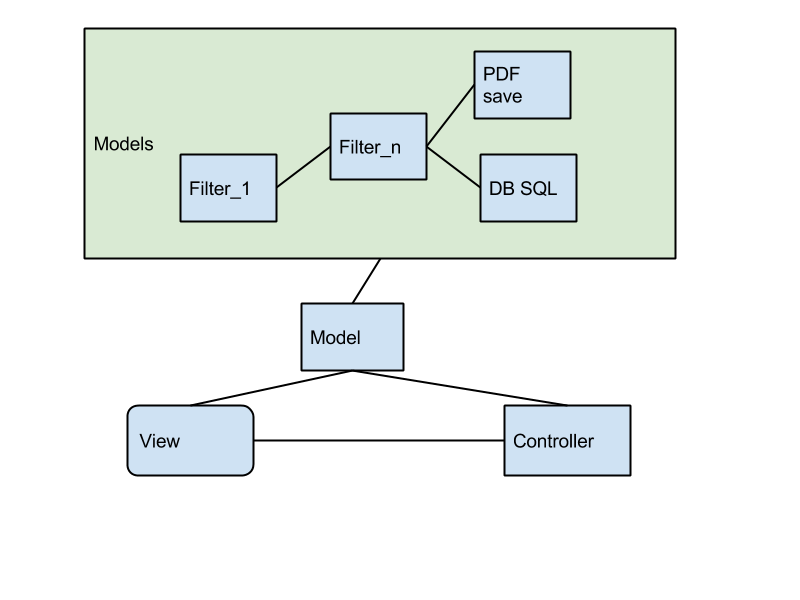
\includegraphics[width=0.8\textwidth]{images/architecture00.png}
\caption{Logical view}
\label{fig:logical_view}
\end{figure}
\newpage

\subsubsection{Scenario view}
\begin{figure}[H]
\centering
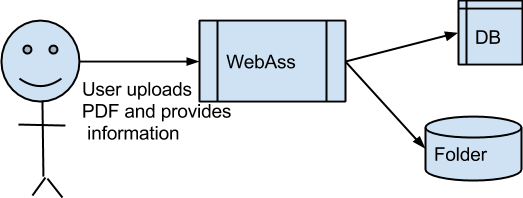
\includegraphics[width=0.8\textwidth]{images/architecture01.png}
\caption{Scenario view}
\label{fig:scenario_view}
\end{figure}




\subsubsection{Physical view}
\begin{figure}[H]
\centering
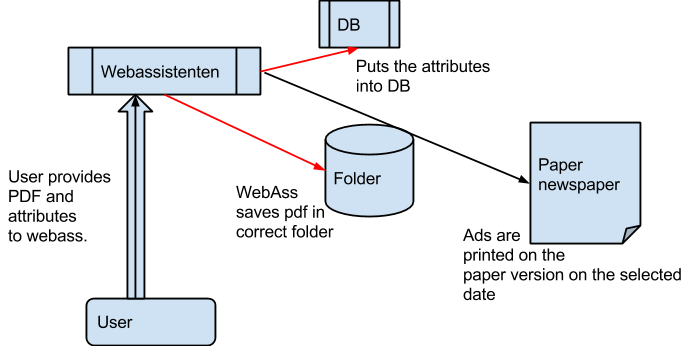
\includegraphics[width=0.8\textwidth]{images/architecture02.png}
\caption{Physical view, we implement the red arrows}
\label{fig:physical_view}
\end{figure}
\newpage
\subsection{Class diagram}
From these views, we made this class diagram.
\begin{figure}[H]
\centering
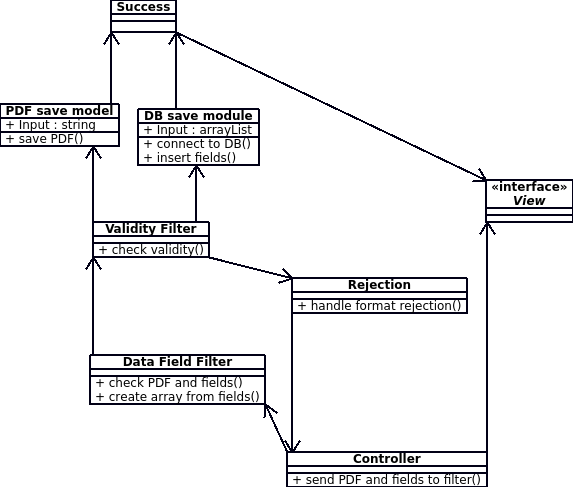
\includegraphics[width=0.8\textwidth]{diagrams/class_diagram.png}
\caption{Digital class diagram}
\label{fig:class_diagram}
\end{figure}
\subsection{Patterns}
MVC due to the technology and pipe \&  filter to filter the data and due to the modifiability requirement.
\subsection{Tactics}
\subsubsection{Modifiability}
\begin{itemize}
\item Increase semantic cohesion
\item Decrease coupling
\item Split modules
\end{itemize}

\subsubsection{Performance}
\begin{itemize}
\item Write optimal code
\end{itemize}

\subsubsection{Availability}
\begin{itemize}
\item Our code should not crash the customer's system, but it's their responsibility that the system is available.
\end{itemize}

\subsubsection{Interoperability}
\begin{itemize}
\item The technology and tools we're using should be sufficient to ensure interoperability.
\end{itemize}

\subsubsection{Readability}
\begin{itemize}
\item We will follow the clean coding principle and use camelCase coding. Refer to \ref{Templates and Standards section} Templates and Standards section on page \pageref{Templates and Standards section}
\end{itemize}

\subsection{Changes to the architecture}
When we started to implement the system we quickly found out that the we had architectural drift because the architecture we designed in the start didn't fit well into the web api framework. After we got an overview of the system we had change the architecture to a MVC pattern. 
\begin{figure}[H]
\centering
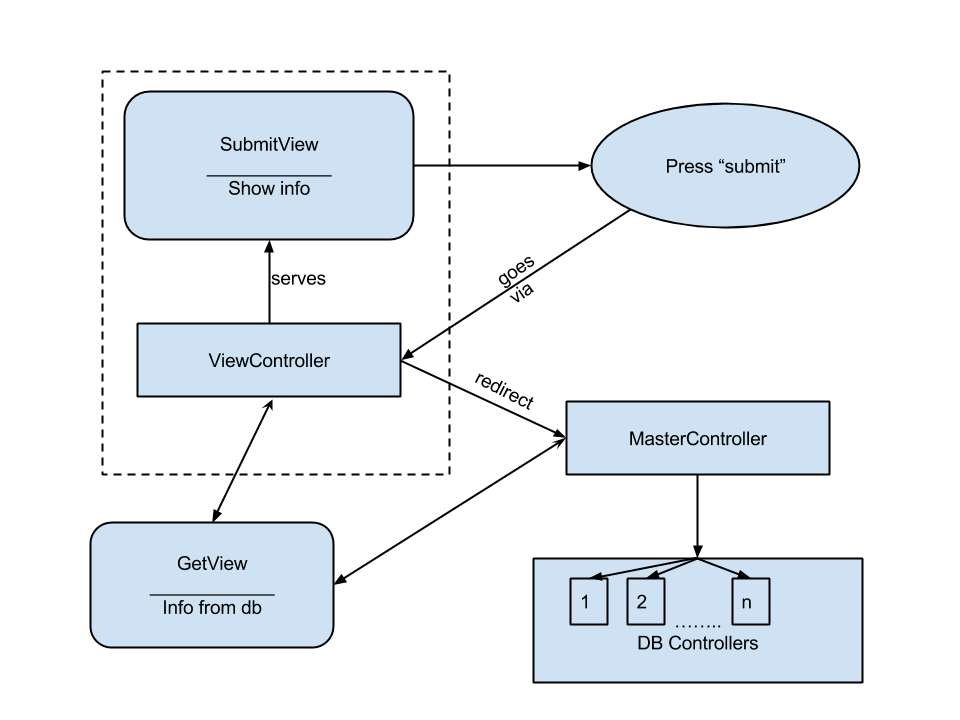
\includegraphics[width=0.8\textwidth]{images/architecture03_revised1.png}
\caption{New diagram showing the information flow}
\label{fig:info_flow}
\end{figure}
We tried to follow this MVC pattern when we implemented the system, however we quickly found out that the getView-Controller was not necessary.
\begin{center}
\begin{figure}[H]
\centering
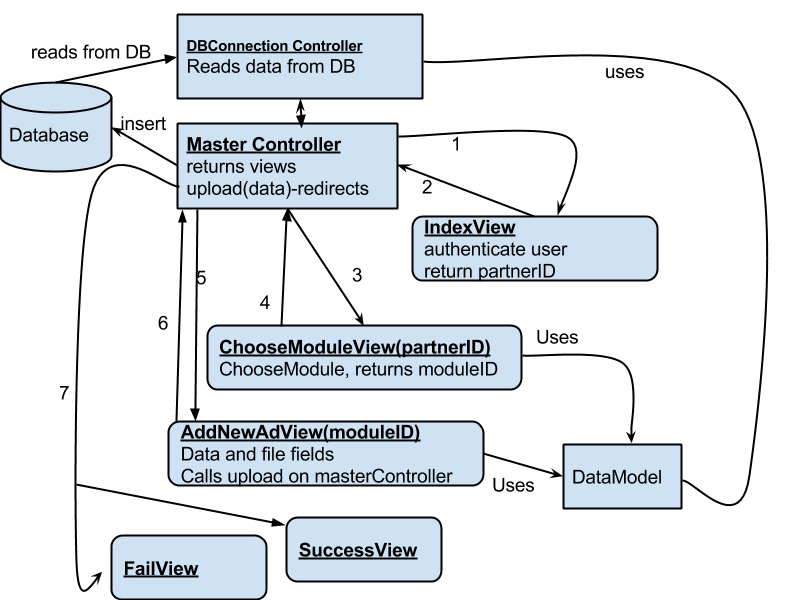
\includegraphics[width=0.8\textwidth]{images/architecture_final01.png}
\caption{The final architecture}
\caption*{6 calls the upload method with files and data\\
7 is the upload method redirecting either to a FailView or a SuccessView}
\label{fig:architecture}
\end{figure}
\end{center}


%Sprints 1-3
\section{Sprint 1}

\subsection{Time Frame}
The time frame for Sprint 1 was week 38 and 39. We started the sprint on September 16th with a weekly supervisor meeting, followed by a sprint plan meeting. We finished the sprint on September 27th with a sprint review meeting.

\subsection{Original Plan}
From our Work Breakdown Structure:
\begin{itemize}
	\item Enable display of available products (no GUI is to be implemented)
	\item Listing the next 5 available booking dates for a selected product
	\item Listing modules available for a selected product
\end{itemize}

\subsection{Revised Plan}
At the sprint plan meeting, we planned the following for this sprint:
\begin{itemize}
	\item Stuff
\end{itemize}

\subsection{Development}
The development started off with the creation of an ASP.NET MVC project. In this project we created data objects for the 

\subsection{Other Work}
In addition to the development, we also completed a draft of the outline for this report and improved on our architectural documentation.

\subsection{Backlog}
What we planned for the sprint that we either did not complete, get time to start, or that was simply pushed back

\subsection{Retrospective}
How we feel about the sprint.
\section{Sprint 2}

\subsection{Time Frame}
The time frame for Sprint 2 was week 40 and 41. We started the sprint on September 30th with a weekly supervisor meeting, followed by a sprint plan meeting. We finished the sprint on October 11th with a sprint review meeting.

\subsection{Original Plan}
From our Work Breakdown Structure, we had the following tasks planned for this sprint:
\begin{itemize}
	\item Receiving pdf-file and save in correct folder
	\item Putting accompanying data in Webassistenten database (table “prospekt”)
	\item Checking accompanying data for required fields
	\item Placing an order in the internal order system
\end{itemize}

Additionally, the following tasks were carried from the previous sprint:
\begin{itemize}
	\item Database connection interface
	\item Database submission logic
\end{itemize}

\subsection{Revised Plan}
At the sprint plan meeting, we planned the following for this sprint:
\begin{itemize}
	\item Set up Entity Framework
	\item Modify start page
	\item Implement saving of pdf-files
	\item Prepare report for midterm delivery
\end{itemize}

\subsection{Development}
At the end of the first sprint, we received a database dump from the customer. The majority of sprint 2 development was centered around setting up a connection to this database through Entity Framework.

Near the end of sprint 2, we realized that we had created the wrong type of project. We had missed the fact that the solution was supposed to use Web API, and had created an MVC project. Some time was therefore spent creating a new Web API project, and porting the code from the previous project into the new one.

\subsection{Other Work}
The deadline for the mid term delivery of the report was originally October 14th, but was at one point in time moved to October 8th. This date coincided with the middle of sprint 2, so a relatively big part of the sprint was spent preparing the report for this delivery. When the deadline was moved back to its original date, more time was spent on improving the report.

\subsection{Backlog}
What we planned for the sprint that we either did not complete, get time to start, or that was simply pushed back.

\subsection{Customer Meeting}
<Add important notes from the customer meeting here, as well as new conclusions made>

\subsection{Retrospective}
<How we feel about the sprint. What we learned, what we are satisfied with, and what we are dissatisfied with.>
\chapter{Sprint 3}

\section{Time Frame}
The time frame for Sprint 3 was week 42 and 43. We started the sprint on October 14th with a weekly supervisor meeting, followed by a sprint plan meeting. We finished the sprint on October 25th with a sprint review meeting.

\section{Original Plan}
From our Work Breakdown Structure:
\begin{itemize}
	\item Database communication interface
	\item Version control system
	\item Bugfixing
	\item Testing
\end{itemize}

\section{Revised Plan}
At the sprint plan meeting, we planned the following for this sprint:
\begin{itemize}
	\item None
\end{itemize}
We had originally planned to be fixing and polishing the finished product, but due to the issues we encountered many of the original planned tasks were pushed to Sprint 3. Sprint 3 thus became a "finish everything that needs to be finished"-Sprint.

\section{Development}
We created the master controller which communicated with the database through the entity framework, it also took care of passing models to the view(s) and handle user request. This master controller was a MVC-type controller which is mostly used as a prototype and for us to test that the data we submit actually reached the system.

\section{Other Work}
After creating and finishing the master controller, the final architecture was made to reflect the implementation of the system. We had architectural erosion due to the framework working differently from what we expected.

The first Friday of this sprint we attended a technical writing course organized by the course staff, where we received pointers on writing our report. These included both general tips as well as concrete improvements for our report specifically.

We started to create the documentation for the customer in Doxygen by XML commenting our code (this was done by adding three slashes "///" in front of all the methods). Doxygen read the implemented code and created the documentation document in HTML. 

\section{Backlog}
Originally we planned to finish the product in Sprint 3, however the we had a lot of issues/problems in both Sprint 1 and 2 so we couldn't start implementing code before Sprint 3. However when the problems were sorted out we actually got down to implementing and communicate with the database. We created a MVC controller of the assignment so we were able to test database connection - insert/select and various other SQL commands via the EF. This MVC controller let us check how the implementation works and gave us a better overview of the framework we were using. However the assignment was to create a Web API controller, so we had to convert it.


\section{Customer Meeting}
We decided to not have a customer meeting for sprint 3 due to our customer Asle not being physically available. Asle was on a 3 weeks vacation in Spain for this period, and we didn't feel the necessity to go to the trouble of setting up a video conference.
However we felt that we had control of the implementation or knew how to fix the issues we stumbled upon. We didn't have much to show either, because we were in the middle of implementing the MVC controller.

\section{Retrospective}
Sprint 3 was a good Sprint for us, we felt that we actually was able to understand the framework and that we actually progressed forward. We was able to communicate with the database, modify rows inside tables, insert data into tables etc.
We also figured out how to serve view (.cshtml) files as webpages through the IIS express by launching the project via VS, and how these views were connected to the controllers. This was enough for us to be able to invoke methods in our controllers, which was heavily used for testing that our written code worked as expected.



\subsection{Tests}

\section{Evaluation}


\section{Conclusion and future work}



\bibliographystyle{plain}
\bibliography{chapters/references/references.bib} 
 
 
%%%Technology
%%%\documentclass[12pt, a4paper]{article} 
 
\usepackage[utf8]{inputenc}
 
 
\usepackage{geometry} % to change the page dimensions
\geometry{a4paper} % or letterpaper (US) or a5paper or....
 
\usepackage{graphicx} % support the \includegraphics command and options
 
\usepackage{booktabs} % for much better looking tables
\usepackage{array} % for better arrays (eg matrices) in maths
\usepackage{paralist} % very flexible & customisable lists (eg. enumerate/itemize, etc.)
\usepackage{verbatim} % adds environment for commenting out blocks of text & for better verbatim
\usepackage{subfig} % make it possible to include more than one captioned figure/table in a single float
% These packages are all incorporated in the memoir class to one degree or another...
 
 
 
\usepackage{amsmath, amssymb}% for mathematical symbols
\usepackage[colorlinks=true,linkcolor=black, urlcolor=blue]{hyperref} % for hyperreferences with black color
%\usepackage[T1]{fontenc} % Uncomment for norwegian document
%\usepackage[norsk]{babel} %
 
%%% HEADERS & FOOTERS
\usepackage{fancyhdr} % This should be set AFTER setting up the page geometry
\pagestyle{fancy} % options: empty , plain , fancy
\renewcommand{\headrulewidth}{0pt} % customise the layout...
\lhead{}\chead{}\rhead{}
\lfoot{}\cfoot{\thepage}\rfoot{}
 
%%% SECTION TITLE APPEARANCE
\usepackage{sectsty}
\allsectionsfont{\sffamily\mdseries\upshape} % (See the fntguide.pdf for font help)
% (This matches ConTeXt defaults)
 
%%% ToC (table of contents) APPEARANCE
\usepackage[nottoc,notlof,notlot]{tocbibind} % Put the bibliography in the ToC
\usepackage[titles,subfigure]{tocloft} % Alter the style of the Table of Contents
\renewcommand{\cftsecfont}{\rmfamily\mdseries\upshape}
\renewcommand{\cftsecpagefont}{\rmfamily\mdseries\upshape} % No bold!

\begin{document}

\section{Technology}

\subsection{Windows 7, 8}
Microsoft Windows 7 and - 8 are operating systems by the Microsoft Corporation. They logically provide good support for .NET developments, seeing as .NET targets the Windows platform and is made by Microsoft. Visual Studio is made for Windows, and was our main IDE, so all team members had access to PCs with Windows installed.

\subsection{Ubuntu Linux}
This OS is perhaps the most widely used distribution of Linux, developed by Canonical Ltd. It provides good support for many development tools, except of course Windows development. However we did find support for using it for some Windows development.
This operating system was used by one team-member on a laptop, when working on-site at NTNU. For coding, Mono with MonoDevelop was used, while other tasks were mostly unaffected. The operating system provides good support for other parts of the process, such as Git and \LaTeX.

\subsection{Mac OSX}
%TODO

\subsection{Visual Studio 2012}
Visual Studio is Microsofts IDE for development for their platforms. This is the main IDE we developed the framework on, seeing as it has very good integration with C\# and .NET platforms, which we were required to use.

\subsection{.NET and Mono}
We were required to use ASP .NET MVC for our framework. ASP .NET MVC is a framework for web applications which enables the use of the Model View Controller (MVC) pattern. It is part of Microsofts .NET Framework suite, which is the preferred way of interactiong with Windows systems and OSes.

Mono is the open source-, cross-platform version of the .NET suite, which we used when not developing on Windows machines. It is available both for Windows, OS X, most Linux Distributions, Android, and various other operating systems.

\subsection{MonoDevelop}
This is an open source IDE for development with Mono, available for OS X and most Linux distributions. This was the IDE used when not developing on Windows machines.

\subsection{LaTeX}
We quickly chose \LaTeX \ for our typesetting. It being the de-facto standard for academic typesetting, with good support for both code snippets, tables, references and bibliography.

Most of our group also had at least some experience using it, and some were quite experienced, which made the choice easier.

\subsection{Git}
For our version control and source repository, we chose Git. This because we had most experience with it, and found it easy to set up via GitHub (where we all had accounts already). It also has the advantage of being distributed, so we could avoid a single point of failure, and having a staging area where one can selectively commit files according to whether they're ready or not, instead of risking accidental changes which might break something.

Both the source code and the entirety of the report source files were stored on GitHub, since both would be catastrophical to lose, and were quite important to have under version control in case we needed to track problematic changes.

\subsection{Trello}
To support our agile process and sprints, we used Trello for planning and control of workflow. It is an online Kanban Board tool, where we can create work packages and issues, while tracking who does what, and tracking backlog, finished modules, and work in progress.

\subsection{Web API}
%TODO

\subsection{Dropbox}
\href{http://www.dropbox.com}{Dropbox} is a syncing service that let you choose a local folder on your machine that will be synced to the cloud. Dropbox lets you share folders and files inside a shared Dropbox folder.

We used Dropbox for sharing and synchronizing internal documents that usually were only useful for a limited time, but might be referenced later.

\subsection{Google Drive}
\href{https://drive.google.com/}{Google Drive} is Google's office pack. The difference between Drive and other office solutions (like Microsoft Office , OpenOffice/LibreOffice) is that Drive exist in the cloud and lets the user simultaneously work on a document.

Google Drive was used for simultaneous collaboration on documents, where the content was up for discussion, or it was advantageous to see what the others where writing.

\end{document}	%%%TODO: Comment in this when technology file is complete, and begindocument is removed

\end{document}